\documentclass[11pt,a4paper]{report}
\usepackage[utf8]{inputenc}
\usepackage[english]{babel}
\usepackage[T1]{fontenc}
\usepackage{amsmath}
\usepackage{amsfonts}
\usepackage{amssymb}
\usepackage{makeidx}
\usepackage{graphicx}
\usepackage{float}
\usepackage{lmodern}
\usepackage{tikz}
\usetikzlibrary{intersections}
\usepackage{pgfplots}
\usetikzlibrary{calc}
\usepackage{geometry}
\geometry{hmargin=2cm,vmargin=2cm}
\usepackage{fancybox}
\usepackage{xcolor}
\usepackage{mathtools}
\usepackage{enumitem}
\usepackage{tcolorbox}
\usepackage{colortbl}
\usepackage{fancybox}
\tcbuselibrary{most}
\usepackage{pifont}
\usepackage{caption}
\usepackage{subcaption}
\usepackage{eso-pic}
\usepackage{nicematrix}
\usepackage{multicol}
\usepackage{booktabs}
\usepackage{svg}
\usepackage{derivative}
\usepackage{wrapfig}
\usepackage{stmaryrd}
\usepackage[backend=biber]{biblatex}
\addbibresource{references.bib}
\author{Andrea}
\setlength{\columnseprule}{0.001 cm}
\setlength{\columnsep}{1cm}
\renewcommand{\thesection}{\Roman{section}}
\renewcommand{\thesubsection}{\arabic{subsection}}
\renewcommand{\thesubsubsection}{\alph{subsubsection}}
\usepackage{amsmath}
\colorlet{shadecolor}{cyan!15}
\usepackage{fancyhdr}
\usepackage{etoolbox}
\usepackage{fourier-orns}
\usepackage{lettrine}
\renewcommand{\headrulewidth}{-10pt}
\usepackage[export]{adjustbox}
\renewcommand{\headrule}{%
\vspace{6pt}\hrulefill
\raisebox{0pt}{\quad\decofourleft\decotwo\decofourright\quad}\hrulefill}
\pagestyle{fancy}
\fancyhf{}
\rhead{ \textcolor{black}{\footnotesize \today}}
\lhead{ENS}
\chead{ \textcolor{black}{· \emph{Lussac Spikesorting Optimization} ·}}
\rfoot{Andrea Combette}
\fancyfoot[C]{\thepage} 
\usepackage{titlesec}
\titleclass{\chapter}{straight}
\titleformat{\chapter}[display]
{\normalfont\bfseries\filcenter}
{\color{black}\LARGE\thechapter}
{1ex}
{\color{black}\titlerule[2pt]
\vspace{2ex}%
\LARGE}
[\vspace{1ex}%
{\titlerule[2pt]}]
\newlength{\tabcont}
\setlength{\parindent}{0.0in}
\setlength{\parskip}{0.05in}
\pgfplotsset{width=7.5cm,height = 6cm,,compat=1.9}

\setcounter{tocdepth}{4}
\setcounter{secnumdepth}{4}

\begin{document}
\begin{titlepage}
    \AddToShipoutPictureBG*{
        \begin{tikzpicture}[overlay,remember picture]
            \draw [line width=3pt]
            ($ (current page.north west) + (2cm,-2.0cm) $)
            rectangle
            ($ (current page.south east) + (-2cm,1.8cm) $);
            \draw [line width=1pt]
            ($ (current page.north west) + (2.15cm,-2.15cm) $)
            rectangle
            ($ (current page.south east) + (-2.15cm,1.95cm) $);
        \end{tikzpicture}
    }
    \begin{center}
        \begin{figure*}
            \begin{center}
                \vspace*{2cm}
            \end{center}
        \end{figure*}
        \rule{14cm}{2pt}\vspace{.7cm}

        \textbf{Supervised research project}

        \vspace{.5cm}
        Supervised by : \textbf{Boris Barbour} and \textbf{Aurélien Wyngaard}

        \rule{14cm}{2pt}\vspace{1cm}
        \vspace{2.5cm}

        \Large Andrea Combette

        \vspace{5cm}

        \raisebox{-5pt}{\quad\decofourleft\decotwo\decofourright\quad}

        \vspace{6cm}

        \begin{minipage}{14cm}
            \small{
                \textbf{Cautionary note :} This paper is a report for an internship, it deals with machine learning approach to tackle spike-sorting problems in neurosciences. It is not intended to be a complete and rigorous study of the subject. The reader is invited to refer to the references for further details.
                It has been made by a Master Student, with some background in physics and mathematics, but no prior knowledge of the subject. It is therefore not intended to be a reference for experts in the field.
            }
        \end{minipage}
    \end{center}
\end{titlepage}

\newpage
\tableofcontents
\newpage
\begin{center}
    \vspace*{1cm}
    \fontsize{11}{13 }\selectfont

    \begin{minipage}{.75\linewidth}
        \chapter{Introduction}

        \lettrine[lines=3]{\color{black} T}{he} study of neural activity at the single-cell level is fundamental to understanding the intricate workings of the brain. Neurons communicate through electrical impulses, or spikes, which necessitate precise detection and classification for comprehensive analysis. These communications are driven by ionic transport between synapses (specific places between dendrites and axon two main components of the neural transmissions).

        \begin{figure}[H]
            \begin{center}
                \hspace*{-1cm}\includegraphics[width=.8\linewidth]{./figure/neuron_anat.jpg}
            \end{center}
            \caption{Neuron anatomy with different components. Neurons are connected each others via axon and dendrites, the neural signal is
                electrical and is due to the polarization of the neuron membrane.}
            \label{fig:}
        \end{figure}


        Understanding which neurons are excited at a given moment allows us to decipher, to a certain extent, the language of our brain. The state of a neuron is defined by the potential of the neuron membrane, and when a neuron is excited, it undergoes what is known as an action potential. The propagation of these action potentials serves as a fundamental basis for comprehending the intricate nature of neural activity.
        In our pursuit to detect and categorize these elusive spikes, we typically employ multiple electrode arrays in tandem with sophisticated classification methods. The classification of neuronal signals, specifically action potentials, constitutes a pivotal domain within neuroscience. It facilitates real-time analysis of cerebral information, providing insights into the motor actions envisioned by the subject. The automation of classification tasks involves the utilization of diverse algorithms, prompting the question of which algorithm is most efficient for classifying neuronal signals. The answer is context-dependent; it varies based on the specifics of the study.
        To enhance our results, envisioning the combination of multiple algorithms for improved classification becomes essential. This is precisely the objective of the Lussac project, which endeavors to amalgamate results from diverse algorithms \cite{Kilosort}.

    \end{minipage}

    \begin{minipage}{.75\linewidth}
        \begin{figure}[H]
            \begin{center}
                \hspace*{-1cm}\includegraphics[width=1.2\linewidth]{./figure/spike.png}
            \end{center}
            \caption{Spikesorting analysis Principles of neurons. The local field potential contains multiple neuron signals, the goal of the spilesorting algorithm is to
                isolate each signal and to attribute each spikes in the local field to a specific neuron. There is many methods to do so. Lussac goal is to deal with multiple of these algorithms to extract the best from each.}
            \label{fig:}
        \end{figure}

        \textbf{Lussac}\cite{Lussac} is a pipeline used for merging and post-processing multiple spike-sorting analyses.
        The goal of this first part is to optimize the decision process, when \textbf{lussac} deals with multiple sorted neurons or analyses, this study is mainly a graph optimization problem,
        with bidirectional link between nodes (nodes are neurons in Lussac study, that are connected each other by multiple metrics).
        Previously, lussac sortings presented some issues with the decision process leading episodically to large neuron clusters $\sim 30$. It means that Lussac is quite sensible to neuron doubloons inside each analysis, to deal with this issue we propose a more traditional approach to the problem, using clustering algorithm outlier detection methods and support vector machine algorithm.
        Previous approach involves testing various methods to identify the most suitable one for each detected neuron using multiple metrics, leading to conclusive outcomes. Another strategy involves the utilization of a machine learning approach to delineate the optimal boundaries between different clusters of neurons and to identify the highest-quality neurons within each cluster.
        The initial segment of this report is dedicated to the examination of neuron classification within specific clusters, utilizing multiple metrics. Each spikesorting algorithm employed by Lussac provides information regarding the detected neurons, necessitating the development of a methodology to integrate these insights for each spikesorting analysis. The subsequent section focuses on evaluating the quality of neurons within each cluster using diverse metrics, ultimately isolating the premier neurons in each cluster.
        Both steps, when combined, provide a comprehensive overview of the quality of the neuron signals, and allows us to build a stronger and efficient spikesorting analysis.

    \end{minipage}
\end{center}
\newpage
\fontsize{12}{13}\selectfont




\begin{multicols}{2}


    \chapter{Lussac sorting: Clustering every group of neurons}

    To Identify which neurons are identical between each analysis, and to process each cluster of the same \emph{real neuron}, we first need to deal with relations between nodes of the Lussac graph.
    To do so, multiple clustering methods can be unearthed applied to multiple type of graph. For example we can cluster neurons together if their connections inside the graph verified some specific properties, like the similarity between both neurons \dots Or we can test clether data structures.
    \section{Clustering on low dimensional space}
    \subsection{Graph Space}
    Given some relations between two nodes, one want to know if this relation is good or not. To do so, we can consider using
    classification regression algorithm to determined if a relation is good or not. This approach is quite simple and general and allows us to know given a fitted model and a new relation if the new relation is good or not.
    First we have to cluster the analyses, neurons coding for the same \emph{real neuron}.
    let's consider the low dimensional space :
    $$\{(p_i^1, p_i^2, p_i^3), p_i \in \llbracket 0,N^2 \rrbracket\}$$ where $N$ is the number of neurons, and $p^i$ the i-th components of the given graph edge.
    Two species clustering is used to determine the class of each edge relation. Here the three components of the edge are the similarity, the template diff and the correlation diff.
    \subsection{Clustering Metrics}
    \subsubsection{Similarity}
    The similarity of two neurons $n_i$ and $n_j$, let's give us $N_{ij}$ the number of coinciding spikes between $n_i$ and $n_j$ and $N_i$ and $N_j$ the number of spikes of $n_i$ and $n_j$ respectively. Then we define the similarity as follows :
    $$\text{sim}(n_i, n_j) = \frac{N_{ij}}{\min (N_i, N_j)}$$

    \subsubsection{Correlogram difference}
    The correlogram difference compares the two neurons autocorellogram, lets'consider both as : $\Gamma_1 $ and $\Gamma_2$ and the cross-correlogram as $\Gamma_{12}$.

    \begin{figure}[H]
        \hspace*{1cm}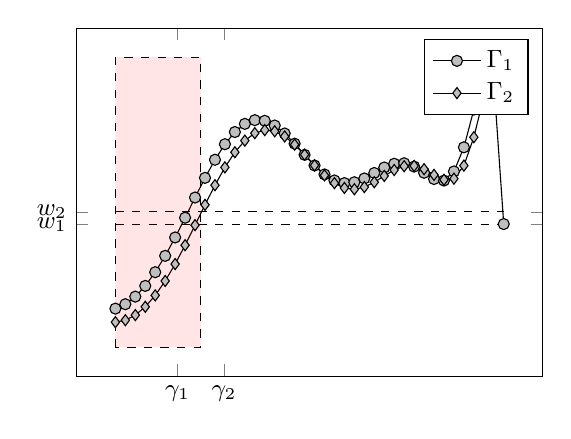
\begin{tikzpicture}
            \tikzstyle{every node}=[font=\small]
            \begin{axis}[
                    legend pos= north east,
                    axis lines = box,
                    ytick={-10,10},
                    yticklabels={$w_1$,$w_2$},
                    xtick={40, 70},
                    xticklabels={$\gamma_1$,$\gamma_2$},
                    variable = t,
                    trig format plots = rad,
                ]



                \addplot [
                    domain= 0:250,
                    samples=40,
                    color=black,
                    mark = *,
                    mark options = {solid, fill=gray!50}
                ]
                {(-140.23437571283273 + 0.6932908290754085 * x ^ 1 + 0.057818025383540146 * x ^ 2 + 0.00016743922300810351 * x ^ 3 -0.000003599158649596702 * x ^ 4 -4.505887859319144e-8 * x ^ 5 + 7.411857043551175e-12 * x ^ 6 + 3.1631082139425804e-12 * x ^ 7 + 6.458290275733523e-15 * x ^ 8 -9.706927463739397e-17 * x ^ 9 -2.4208716299110894e-19 * x ^ 10 + 1.3755743234698024e-21 * x ^ 11 + 3.5494284276047266e-24 * x ^ 12 -7.355158274790618e-27 * x ^ 13 -1.8894648875025586e-29 * x ^ 14)};
                \addlegendentry{$\Gamma_1$};


                \addplot [
                    domain= 0:250,
                    samples=40,
                    color=black,
                    mark = diamond*,
                    mark options = {solid, fill=gray!50}
                ]
                {(-159.23437571283273 + 0.6832908290754085 * (x-5) ^ 1 + 0.058318025383540146 * (x-5) ^ 2 + 0.00016743922300810351 * (x-5) ^ 3 -0.000003599158649596702 * (x-5) ^ 4 -4.505887859319144e-8 * (x-5) ^ 5 + 7.411857043551175e-12 * (x-5) ^ 6 + 3.1631082139425804e-12 * (x-5) ^ 7 + 6.458290275733523e-15 * (x-5) ^ 8 -9.706927463739397e-17 * (x-5) ^ 9 -2.4208716299110894e-19 * (x-5) ^ 10 + 1.3755743234698024e-21 * (x-5) ^ 11 + 3.5494284276047266e-24 * (x-5) ^ 12 -7.355158274790618e-27 * (x-5) ^ 13 -1.8894648875025586e-29 * (x-5) ^ 14)};
                \addlegendentry{$\Gamma_2$};

                \addplot [
                    dashed,
                    domain=-0:250,
                    samples=100,
                    color=black,
                ]
                coordinates {(0, 10) (250, 10)};

                \addplot [
                    dashed,
                    domain=0:250,
                    samples=100,
                    color=black,
                ]
                coordinates {(0, -10) (250, -10)};

                \addplot [
                    dashed,
                    domain=-100:-50,
                    samples=100,
                    fill=red,
                    fill opacity=0.1,
                ]
                coordinates {(0, -200) (0, 250) (55, 250) (55, -200) (0, -200)};
            \end{axis}
        \end{tikzpicture}
        \captionsetup{justification=centering, margin={2cm, 1cm}}
        \caption{Correlogram difference overview}
        \label{fig:corr}
    \end{figure}

    The following parameters $w_1, w_2, \gamma_1, \gamma_2$ are used to determine the most relevant range of the correlogram.
    $\gamma_i$ is defined as the first annulation of the second derivative of $\Gamma_i$. Finally the correlogram difference is computed wih $\Gamma_1, \Gamma_2, \Gamma_{12}$ restricted to $[\gamma_1, \gamma_2]$.
    $$\text{corr}_i = \frac{|\Gamma_i - \Gamma_{ij}|}{w_j - w_i}$$
    Then we take a ponderated mean of the correlation difference of both neurons.
    \subsubsection{Template difference} For the template difference, it's just a simple euclidean distance between the two templates, devided by the sum of the absolute value of the two templates. The so called template, refers to the waveform of the extracted neuron from the raw signal (fig 1.2)

    \subsubsection{Asymmetric similarity}

    Let's consider two spiking neurons, $n_1$ and $n_2$, we define the asymmetric similarity as follows :

    $$\text{sim}(n_i, n_j) = \frac{N_{ij}}{N_i}$$
    Hence, even if a neuron is learned lately by the algorithm, it will be able to be classified as a good neuron, if it has a lot of coinciding spikes with a neuron already learned.
    \subsubsection{Cross-contamination of neurons}

    The contamination \cite{Contamination} gives a corrected number of violations metrics, it's caculated using a censure time. Indeed spike sorters are not able to detect spikes that are too close to each other. A way of correct the rate of number of violation is to not consider a specific time window around each spike. This time window is called the censure time.


    \subsection{Unsupervised Clustering}

    Unsupervised clustering is a method of clustering that does not require the user to specify the number of clusters to be generated. Instead, the algorithm itself will determine the optimal number of clusters based on the data.
    For this tasks we will use a KMEANS algorithm specifying 2 classes, to isolate good relations. Kmeans is a method of vector quantization, originally from signal processing, that aims to partition n observations into k clusters in which each observation belongs to the cluster with the nearest mean (cluster centers or cluster centroid), serving as a prototype of the cluster.

    \begin{figure}[H]
        \centering
        \includegraphics[width=\linewidth]{./figure/param_space_km.png}
    \end{figure}
    \captionof{figure}{We omit the dependence over the template difference for vizualizations. Big circles are the ground truth label, red one are known good relations between neurons (i.e they are in the same cluster, and blue one are bad ones. The results of the unsupervised clustering is
        represented by the little blue and red circle, the red one are the good relations, and the blue one are the bad ones. The unsupervised clustering is not able to separate the data in a good way.)}

    Despite the fact that Kmeans algorithm are robust and highly generalizable. The clustering is far from being efficient, indeed due to the large spread of data in the template diff the clustering is not able to separate the data in a good way for the similarity axis.
    And the continuum of points in the (similarity, temp diff) plane prevents us from a good discrimination. To solve this issue we could have tweaked the sample weighting parameter of the KMeans algorithm as we will further. But to get more control on the learning process of the algorithm, we can use a supervised clustering algorithm, which will be able to separate the data in a more efficient way.
    \subsection{Supervised Clustering}
    Here the idea is to first use a classification methods to first determine if the edge is good or not, given the edge relation for each node's edges. Then we can create clusters, using the validity
    of the edge's relations. To do so we use a support vector machine classifier, which is a supervised learning model, i.e. it requires a training set of labeled data to learn from. The goal of the SVM is to find the insights of this algorithm will be discussed in the next part.
    \subsubsection{Support Vector Machine Classifier}
    \paragraph{Principle}
    The support vector machine \cite{kernel} classifier is a supervised learning algorithm that can be used for both classification or regression challenges. However, it is mostly used in classification problems.
    In this algorithm, we plot each data item as a point in n-dimensional space (where n is the number of features you have) with the value of each feature being the value of a particular coordinate.
    Then, we perform classification by finding the hyper-plane that differentiate the two classes very well. This hyper-plane is called as the margin. The SVM classifier finds the optimal margin.


    This method allows us to tackled non-linearly separable data, by introducing the kernel trick, which consists in mapping the data into a higher dimensional space, where the data will be linearly separable. For example,
    we can use a radial basis function kernel, to fit Gaussian distribution values to the data.
    $$K(x_i, x_j) = \exp(-\gamma ||x_i - x_j||^2)$$
    \paragraph{Application}
    Here the SVM will be simply parametrized by a linear kernel and applied on the lussac graph relations to isolate neurons clusters.
    \begin{figure}[H]
        \includegraphics[width = .98\linewidth]{./figure/param_distrib.png}
    \end{figure}
    \captionof{figure}{Neurons relations distributions for identical clusters, like we said before, the distributions for the correlogram and the template are quite similar,
        as opposed to the similarity distribution. Hence, the goal is to separate these 3 distribution in an optimal way, this is why we will limit our visualizations to the similarity and the template difference.}

    \begin{figure}[H]
        \includegraphics[scale = 1]{./figure/decision_function.png}
        \caption{Decision Function for the given SVM, the correlation dependence is omitted due to its weak impact on the decision boundaries.  Here the SVM is able to separate the data in a good way, we reach a score of 0.9997 for the relation's classification, we can see that good relations colored in red are mostly to the right of the boundary and bad (in blue) relations to the left. However this high score must be taken with a grain of salt, indeed there is a lot of bad relations inside the data,
            and their classification is not really relevant, since this it is quite obvious that they don't belong to the same neuron. The introduction of a relative metrics should solve this issue and will be introduced further.}
    \end{figure}

    \begin{figure}[H]
        \includegraphics[scale = 1]{./figure/cluster_length.png}
        \vspace{0.15cm}
    \end{figure}
    \captionof{figure}{Here we can see the length histogram of the clusters, the length of the clusters is the number of neurons inside this latter. In blue the predicted cluster length and in red the true one. We can see that, these two distributions are quite similar, which is a good sign, one can lays the emphasis on the fact that predicted clusters tend to have smaller size, which is quite relevant since it eliminates the risk of having a large cluster containing multiple neurons, creating really small clusters of bad units.}


    \subsection{Clustering Efficiency}  Hence the labelling is different from the Lussac, one have
    to define another score method to quantify the clustering quality. We propose the following formula :

    $$ \text{score}(Y^{\text{pred}}, Y^{\text{true}}) = \sum_{k=0}^N \frac{ \# (G_k^{\text{pred}} \cap  G_k^{\text{true}})}{\max (\# G_k^{\text{pred}}, \# G_k^{\text{true}})}$$

    with $G_k$ the $k$-th subset of neighbors index deduced from the clustering $G_k^{\text{pred}}$ method and lussac analyses for $G_k^{\text{true}}$. Thanks to this metrics we are able to avoid the labelling problem,
    and we can evaluate the clustering quality in a more efficient way. It satisfies the following properties :
    $$\begin{cases}
            score(Y,Y) = 1                     \\
            score(Y, \emptyset) = 0            \\
            score(Y_1, Y_2) =  score(Y_2, Y_1) \\
        \end{cases}$$

    \section{Clustering on high dimensional space}
    Next we will just keep the similarity, template difference, correlogram difference metrics to simplify the problem. The features space is then of dimension 3.
    Let's consider the high dimensional space :

    $$\{p_i^j, i,j \in \llbracket 0, N \rrbracket \times \llbracket 0,3 N \rrbracket\}$$ where $N$ is the number of neurons, and $p^i$ the i-th components of the given graph edge.
    Two species clustering is used to determine the class of each edge relation. Hence, the dataset has the following shape :
    $$
        \underbrace{
            \begin{pmatrix}
                |1,0,0| & \dots   & \dots   \\
                \dots   & |1,0,0| & \dots   \\
                \dots   & \dots   & |1,0,0| \\
            \end{pmatrix}}_{3N}
    $$
    In this representation we do not consider the link validity but how the neuron are connected together, this point of view increase drastically dimensions, but it allows us
    to discriminate the data in a much more comfortable way. The idea behind this representation is that, to connected neurons on the graph should have the same edges coordinates in this space. Because
    they share the same properties (similarity, template diff, corr diff)
    The unsupervised clustering of this dataset provides $n_{\text{pred}}$ clusters. We use the same metrics as before to evaluate the clustering quality. Then when the model is fitted, we can use it to predict is a new node inside the Lussac graph is inside another cluster.

    \subsection{Various unsupervised clustering algorithms}


    \begin{itemize}
        \item \textbf{Affinity propagation}
              AffinityPropagation creates clusters by sending messages between pairs of samples until convergence.
              A dataset is then described using a small number of exemplars, which are identified as those most representative of other samples.
              The messages sent between pairs represent the suitability for one sample to be the exemplar of the other, which is updated in response to the values from other pairs.
              This updating happens iteratively until convergence,
              at which point the final exemplars are chosen, and hence the final clustering is given.

        \item \textbf{HDBSCAN}
              Hierarchical Density-Based Spatial Clustering of Applications with Noise. Performs DBSCAN over varying epsilon values and integrates the result to find a
              clustering that gives the best stability over epsilon. This allows HDBSCAN to find clusters of varying densities (unlike DBSCAN), and be more robust to parameter selection
    \end{itemize}
    \subsection{Results}
    \subsubsection{Affinity Propagation Results}
    The vizualizations of the created graphs are omitted due to the large number of clusters created by the algorithm. The best score obtained after a simple gridsearch relative to the clustering is 0.687, which is quite low, and cannot be compared to the previous clustering methods.
    \begin{figure}[H]
        \centering
        \includegraphics[width=0.98\linewidth]{./figure/cluster_length_ap.png}
        \caption{Here we can see the main reasons of the low clustering score. It's mainly due to multiple single clusters, which were normally from medium size clusters, which is not really relevant since we want to ge rid of big clusters.}
        \label{fig:}
    \end{figure}

    \subsubsection{HDBSCAN Results}
    For the HDBSCAN algorithm, we obtain a score of 0.78, which is too low compared with the previous results, the conclusion are the same than for the affinity propagation algorithm, the main reason of the low score is the presence of multiple single clusters, which were normally from medium size clusters, which is not really relevant since we want to ge rid of big clusters.
    \chapter{Nodes clustering}

    \subsection{Node Space}
    The second clustering is based on the study of the space of neurons quality metrics. The goal of this process is to eliminate bad neurons in the previously defined clusters.



    \subsection{Different Methods}
    \subsubsection{Metrics Overview}
    \begin{itemize}
        \item \textbf{rb contamination} : The contamination gives a corrected number of violations metrics, indeed it's calculated using a censure time. Indeed, spike sorters are not able to detect spikes that are too close to each other. A way of correct the rate of number of violation is to not consider a specific time window around each spike. This time window is called the censure time.
        \item \textbf{SNR} : The SNR is the ratio between the mean of the spike amplitude and the standard deviation of the noise. The SNR is a measure of the quality of the spike detection. A high SNR means that the spike detection is good.
        \item \textbf{presence ratio} : The presence ratio is the ratio between the number of spikes detected and the number of spikes expected. A high presence ratio means that the spike detection is good.
        \item \textbf{firing rate} : The firing rate is the number of spikes detected divided by the duration of the recording. A high firing rate means that the spike detection is good.
        \item \textbf{synchrony} : The synchrony is the ratio between the number of coinciding spikes and the number of spikes detected. A high synchrony means that the spike detection is good.
        \item \textbf{sd ratio} : The sd ratio is the ratio between the standard deviation of the spike amplitude and the standard deviation of the noise. A high sd ratio means that the spike detection is good.
        \item  \textbf{quality score metrics} :  The quality metrics is score taking into account the contamination and the number of spikes (firing rate). It is defined as following :
              $$S = N(1 - (k+1)C)$$ witth $N$ the number of spikes, $C$ the contamination and $k$ a constant. Generally we take $k = 1$ for minimizing the accuracy, but one could argue that it's not the best choice, indeed a false positive has a stronger impact on the spike sorting quality,
              so we could take $k = 2.5$ to accentuate the dependence of false positive on the score. Indeed, the former formula leads to : $$S = N - FN - k FP$$.
    \end{itemize}
    To have deeper insigths, we sould explore the correlations between the different metrics, one common way in machine learning is to use the Person correlation coefficient, which is defined as follows :
    $$\rho_{X,Y}  = \frac{\text{cov}(X,Y)}{\sigma_X\sigma_Y}$$ with $\text{cov}(X,Y)$ the covariance between $X$ and $Y$ and $\sigma_X$ and $\sigma_Y$ the standard deviation of $X$ and $Y$ respectively.
    It's really usefull to determinate a dependancy between metrics, and to isolae indepedant ones. Indeed if the pearson correlations close to 0, then the metrics are independant, the goal of this is to find the most relevant metrics for the clustering.

    \begin{figure}[H]
        \centering
        \includegraphics[width=\linewidth]{./figure/correlation.png}
        \caption{Correlation matrix of the different metrics, we can see that the firing rate and the presence ratio are highly correlated, hence we can drop one of them. The sd ratio and the SNR are also highly correlated, we can drop one of them. The synchrony and the contamination are also highly correlated, we can drop one of them.}
        \label{}
    \end{figure}
    Dropping the cluster dependence allows us to use all the nodes for the global clustering, which should make our predictions more reliable. However some metrics are theorically cluster dependant, some we must drop them, there are the following :
    (firing rate, sd ratio, quality core metrics,)
    For the clustering we use weighted samples for getting rid of the unbalanced dataset problem. Indeed, if we want to isolate the best neuron for each cluster, we have to diminich the impact of other good neurons in the clustering process.
    To do so we first use the following weighting function, of the form :
    $$f(x) = \left[\tanh \left( \frac{x - \text{max}_c /C}{\sigma} \right) + \frac{1}{2} \right]^2$$
    \begin{figure}[H]
        \begin{tikzpicture}
            \begin{axis}[
                legend pos=north east,
                title=Weighting Function,
                axis lines = box,
                xlabel = $x$,
                ylabel = $y$,
                variable = t,
                trig format plots = rad,
                xtick={0.7},
                xticklabel={$\text{max}_{\text{c}}$},
                ]
                \addplot[smooth][
                    domain=0:.68,
                    samples=70,
                    color=black,
                ]
                {tanh(-(x-.4)/.1)/2 + 1/2};
                \addplot [black, mark = text, text mark = $[$ ,every node near coord/.style={anchor=180}] coordinates {( .68, 0)};
                \addplot [black, mark = * ,every node near coord/.style={anchor=180}] coordinates {( .7, 1)};
            \end{axis}
        \end{tikzpicture}
        \caption{Weighting function used for the clustering, the goal is to have a strong impact on the data that are close to the maximum of the cluster, and a weak impact on the data that are far from the maximum of the cluster.}
    \end{figure}
    \subsection{Clustering on every nodes}
    Here we are clustering on every nodes, independantly from their clusters, one strong limitations is that we cannot used metrics that are neuron-dependant, indeed each cluster should encode one single neuron, which has some
    specific property. Hence, we use just the 3 following metrics : snr, contamination, presence ratio :
    \begin{figure}[H]
        \centering
        \includegraphics[width=0.9\linewidth]{figure/decision_function_working_2.png}
        \caption{The data is impossible to separate into 2 clusters : one for good neurons and the other for the bad ones. Hence the SVM is clearly overfitting the data.}
        \label{}
    \end{figure}
    Dropping the presence ratio which appear to be constant for a majority of the nodes, we obtain the following results :
    \begin{figure}[H]
        \centering
        \includegraphics[width=0.9\linewidth]{figure/decision_function_working_3.png}
        \caption{Here the results leads us to the same conclusion as before.}
        \label{}
    \end{figure}
    It's clear that there is a necessity to introduce relative metrics, to have clusters independent results. How data can be relative to clusters,
    one easy way to solve this problem is to renormalize the parameter by the mean and the std of the cluster. Given the following formula :
    $$\frac{p_i - \mu}{\sigma}$$ with i the index of the feature and $p,\mu,\sigma$ the parameter, the mean and the standard deviation for each cluster. Besides the needs
    to have constant spreading of the data appears,indeed here we are studying the 2d case, but the introduction of new parameter should cause some
    issues without this renormalization. This gives the following renormalized distribution.

    \begin{figure}[H]
        \centering
        \includegraphics[width=0.9\linewidth]{figure/clusters_weights.png}
        \caption{Here we introduce the distance weighting defined above. In black, the so-called bad neurons, and in red the best neuron (defined by their accuracy over the ground truth neuron) for each cluster.
            It seems that, thanks to the renormalization, the data can be separated in a good way.}
        \label{}

    \end{figure}

    \subsection{Clustering with relative metrics}
    \subsubsection{Support Vector Machine Classifier}

    However, we can't apply directly this classifier to the clustering problem, indeed we have a strong unbalanced dataset, between the two classes, hence we have rectification coefficient for the weight of each class, to avoid a huge influence of the majority class in the clustering.
    To sum up we have two weighting coefficient, one for the distance and one for the class. The coefficient introduced are (0.5, 5) respectively for the majority class and for the minority class.

    \begin{figure}[H]
        \centering
        \includegraphics[width=0.9\linewidth]{figure/decision_function_working_6.png}
        \caption{On this clustering thanks to the renormalization we got more homogenous separation (solid black line stands for place where the algorithm tends to label points as good neurons and dashed line where the algorithm classifies the neurons as bad), though the clustering method has overfited the data, hence we must try to choose the optimal $\Gamma$ Kernel coefficient in order to have a fixed width of cluster. And to try different penalty parameter to get rid,
            of the noisy data influence inside the clusters of relevant neurons}
        \label{}
    \end{figure}
    Next we perform a grid search to find the optimal gamma and C parameters, this leads to the following results
    \begin{figure}[H]
        \centering
        \includegraphics[width=0.9\linewidth]{figure/grid_search.png}
    \end{figure}
    \captionof{figure}{Here it appears that the optimal parameters are high gamma and high C, however, let's note that this leads to high overfitting, hence we should try to find the optimal parameters, considering that a generalization will lead to a relatively smooth separtaion line : Indeed,
        let's check the shape of the level 0 of the decision function.}
    For the following figures we projected the classifier on the planes of interests for all the metrics. This gives a quick overview of the classifier behaviour in high dimensions.
    Note that without any projections, the classifiers will have better insights of the data, leading to better results, though we cannot plot 7 dimensions data.

\end{multicols}

\begin{figure}[H]
    \centering
    \includegraphics[width=0.9\linewidth]{figure/decision.png}
\end{figure}
\captionof{figure}{Here we try to classify the data, using the optimal parameter used for the grid-search, however, it appears, as expected, that the boundary is totally messing.
    Hence, we must choose small $\Gamma$ as studied before to keep, a relatively smooth boundary. Behind, this required smooth boundaries is the generalization issue, and to have simple rules to know if the neuron is good or not. Even if this much more sophisticated boundaries are probably,
    encoding more simple boundaries inside. To do so we will fix the $\Gamma$ parameter to an arbitrary low number and play with the penalty parameter in order to maximize the clustering score of the method. }
\newpage
\begin{multicols}{2}

    \begin{figure}[H]
        \centering
        \includegraphics[width=0.9\linewidth]{figure/decision_function_working_5.png}
    \end{figure}
    \captionof{figure}{Here we choose $\Gamma = 0.03$ and $C = 1$ (i.e. no penalty), we can see that the clustering is more relevant, but we still have some noisy data inside the clusters, that we can get rid of playing with the penalty parameter. However, one can notice that
        with the base score function, as we discretized the label, we will have some really low score (around 0.4), the need to introduce a new metrics score appears. We propose to use the same weighting as before with a strengthened impact of critically low accuracy, introducing relative accuracy of the cluster into the computation of the score.}

    \begin{figure}[H]
        \centering
        \includegraphics[width=\linewidth]{figure/score.png}
        \caption{Score maximization using $\gamma = .003$ of the coefficient parameter of the weighting function and the penalty paramter of the fiting process, However let's denote the following properties of support vector machine, the C parameter determinates how smooth is the speration curve, for high C the model try to classify all the data correctly, but it can lead to overfitting, for low C the model try to find the largest margin possible, but it can lead to underfitting. Hence we should try to find the optimal C parameter, considering that a generalization will lead to a relatively smooth separtaion line :}
        \label{}
    \end{figure}

    Next we perform a grid search to find the optimal weighting coefficient and $C$ parameters, this leads to the following choice : $\Gamma = 0.03$, $C = 5$, $W_c = 5$ for the weighting coefficient.
    After fitting the model with these parameters we  reached a score of 0.84, which is quite good.

    \subsubsection{Naive Bayes Classifier}
    \paragraph{Principle}
    Naive Bayes classifiers are a family of simple "probabilistic classifiers" \cite{GaussianBayes} based on applying Bayes' theorem with strong (naive) independence assumptions between the features.
    Given a class variable $y$ and a dependent feature vector $x_1$ through $x_n$, Bayes' theorem states the following relationship:
    $$P(y | x_1, \dots, x_n) = \frac{P(y) P(x_1, \dots, x_n | y)}{P(x_1, \dots, x_n)}$$
    \paragraph{Gaussian Naive Bayes}
    In Gaussian Naive Bayes, continuous values associated with each feature are assumed to be distributed according to a Gaussian distribution.
    When we apply the algortithm to our dataset, we obtain the following results :

    \begin{figure}[H]
        \centering
        \includegraphics[width=0.9\linewidth]{figure/cluster_GaussianNB.png}
        \caption{For the 2D clustering on \textbf{synchrony} and \textbf{SNR} we obtained quite good separation line between both clusters of good and bad neurons. This simple separation ilne, has been obtained introducing the same weighting methods used for SVM, except for the class weighting. However for the score evaluation, we implemented this weighting to get rid of the over influence of bad neurons.}
        \label{}
    \end{figure}
    To have deeper insights on the multidimensional clustering we proposed to use the same visualizations as before, with the projections on all metrics planes. This leads to the following :

\end{multicols}
\begin{figure}[H]
    \centering
    \includegraphics[width=0.9\linewidth]{./figure/Gaussian_pair .png}
\end{figure}
\captionof{figure}{Here we plot, the separation line of both clusters, in orange good neurons and in blue bad ones. The diagonal shows the distribution of both types of neuron. One can notice, that for some dimensions the clustering is inefficient. However, results are quite intersesting and the multidimensional analysis leads to a global score of 0.87, given the weighting metrics.}
\begin{multicols}{2}
    \subsubsection{Quadratic Discriminant Analysis}
    \paragraph{Principle}
    Quadratic Discriminant Analysis (QDA) \cite{qda} is a classification algorithm that assumes that the probability density function of the features given the class follows a Gaussian distribution.
    QDA is a simple extension of LDA to a non-linear decision boundary.QDA can be derived from simple probabilistic models which model the class conditional distribution of the data
    for each class. Predictions can then be obtained by using Bayes’ rule, for each training sample $x \in \mathbb{R}^d$ and class $k \in \{1, \dots, K\}$:

    \begin{align*}
        P(X|y=k) & = \frac{P(x|y =k)P(y=k)}{P(x)}                        \\
                 & = \frac{P(x|y = k)P(y = k)}{\sum_lP(X|y = l)P(y = l)}
    \end{align*}


    The idea is then to select the class k which maximizes this posterior probability.

    More specifically,for quadratic discriminant analysis, $P(X|y = k)$
    is modeled as a multivariate Gaussian distribution with density:
    \begin{multline*}
        P(x|y = k) = \frac{1}{(2\pi)|\sum_k|}\exp(-\tfrac{1}{2}(x - \mu_k)^t \\
        (\sum_k-1(x - \mu_k)))
    \end{multline*}
    Here $\sigma_k$ stands for the covariance matrix, the exponential term is the \emph{Mahalanobis} distance between $x$ and $\mu_k$. And $d$ is the umber of features. The only difference with LDA (linear discriminant analysis) is that we do not assume that the covariance matrix is the same for all classes.
    \paragraph{Results Discriminant Analysis}
    When we apply the algortithm to our dataset, we obtained the following results :

    \begin{figure}[H]
        \centering
        \includegraphics[width=0.9\linewidth]{figure/cluster_qda2.png}
    \end{figure}
    \captionof{figure}{The Discriminant analysis leads quite to the same results as for the Bayesian approach (for \textbf{synchrony} and \textbf{SNR}), which was intended, however one can show that the boundaries are a little less strict, and can be expanded a little beyond the Bayesian classifier ones. Whereas, the weighting is exactly the same, even for the score function.}

\end{multicols}
\begin{figure}[H]
    \centering
    \includegraphics[width=0.9\linewidth]{figure/qda_pair.png}
\end{figure}
\captionof{figure}{    For the multidimensional projections study we got the following results : The separation line between both clusters, is indeed larger with the quadratic determinant analysis than for Bayesian analysis. Note that the results seems also quite relevant, since the global analysis, leads to a score of 0.88.}
\begin{multicols}{2}
    \subsubsection{Comparison}
    The three methods for the node's classification seem to be working. One can say that we must take the methods with the best score, to evaluate if a neuron is good or not, we could aolso argue that we must choose the method with the more restrictive decision line, in order to increase the chance to have better neurons. But in this case, we will miss some neurons, which will lead to false negative in the \textbf{analysis}.
    In fact it's not really important to  classify a \emph{bad} neurons which has good metrics as good, since in all cases we must take the best neurons in the cluster. To do so, we propose the following method : When we classify a cluster of neurons, if there are good neurons, we take the nearest neuron from the \textbf{centroid} of the \emph{good} neuron distribution (normalized).
    \begin{figure}[H]
        \centering
        \includegraphics[width=0.9\linewidth]{figure/cluster_choice.png}
        \caption{Centroid method for choosing the best neurons in the case there is many.}

    \end{figure}

    The best score methods, with quite large boundaries is the quadratic determinant analysis, this is why it's the more appropriate to tackle this classification problem.

    \chapter*{Conclusion}
    In this comprehensive study, we have explored various clustering and classification methodologies for the analysis of neuronal data, particularly focusing on spike sorting in neuroscience. The first part, focused on the clustering of same detected neurons my multiple analysis, the second part unearthed the complexity of choosing the best analysis, to provide the best data. Our investigation encompassed unsupervised clustering using KMEANS and hierarchical clustering algorithms, revealing the limitations of these methods in efficiently separating data due to the inherent complexity and spread of the feature space.

    To address the shortcomings observed in unsupervised clustering, we introduced supervised approaches, leveraging Support Vector Machine (SVM), Naive Bayes Classifier, and Quadratic Discriminant Analysis. The SVM demonstrated robustness and generalizability, effectively discerning between good and bad neuronal relations. Notably, the introduction of relative metrics and a weighted scoring system facilitated a more nuanced evaluation, offering insights into the clustering quality.
    The Quadratic Discriminant Analysis emerged as the most promising method, achieving a high clustering score and demonstrating stringent decision boundaries. We proposed a practical approach for selecting the best neurons within a cluster, prioritizing those nearest to the centroid of the good neuron distribution.

    Our findings not only shed light on the challenges associated with traditional clustering methods in the context of spike sorting but also present a novel and effective framework for improved classification. The integration of sophisticated machine learning techniques, coupled with thoughtful metric considerations, provides a promising avenue for advancing the accuracy and efficiency of neuron categorization.

    This study contributes valuable insights into the realm of neuroscience and spike sorting, offering a methodological foundation for future research aimed at enhancing the understanding and analysis of neuronal data. The proposed approaches hold significant potential for application in real-world scenarios, paving the way for more reliable and precise spike sorting methodologies in neuroscientific studies.
\end{multicols}
\printbibliography
\end{document}
